\documentclass[border=5pt]{standalone}
\usepackage[T1]{fontenc}
\usepackage{lmodern,amsmath}
\usepackage[american]{circuitikz}
\usetikzlibrary{arrows.meta,patterns}
\newcommand{\dd}{\mathrm{d}}
\begin{document}
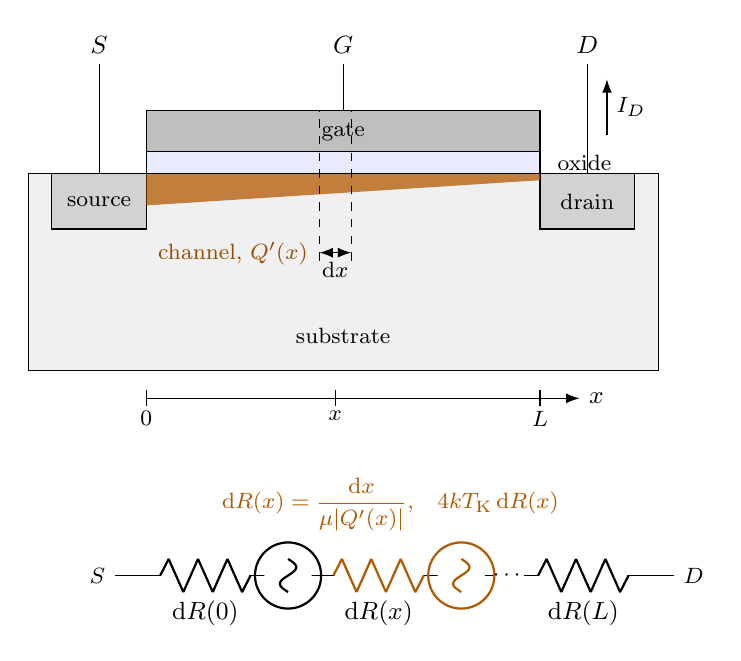
\begin{tikzpicture}[font=\small,>=Latex]
% substrate
\fill[gray!12] (0,0) rectangle (8,2.5);
\draw (0,0) rectangle (8,2.5);
\node[font=\footnotesize] at (4,0.45) {substrate};
% source and drain
\fill[gray!35] (0.3,1.8) rectangle (1.5,2.5);
\fill[gray!35] (6.5,1.8) rectangle (7.7,2.5);
\draw (0.3,1.8) rectangle (1.5,2.5);
\draw (6.5,1.8) rectangle (7.7,2.5);
\node[font=\footnotesize] at (0.9,2.15) {source};
\node[font=\footnotesize] at (7.1,2.15) {drain};
% channel charge, tapering from source to drain
\fill[orange!70!black,opacity=.75] (1.5,2.5) -- (6.5,2.5) -- (6.5,2.42) -- (1.5,2.1) -- cycle;
\node[font=\footnotesize,orange!60!black,anchor=north] at (2.6,1.75) {channel, $Q'(x)$};
% oxide and gate
\fill[blue!8] (1.5,2.5) rectangle (6.5,2.78);
\draw (1.5,2.5) rectangle (6.5,2.78);
\node[font=\footnotesize,anchor=west] at (6.6,2.64) {oxide};
\fill[gray!50] (1.5,2.78) rectangle (6.5,3.3);
\draw (1.5,2.78) rectangle (6.5,3.3);
\node[font=\footnotesize] at (4,3.04) {gate};
% terminals
\draw (0.9,2.5) -- (0.9,3.9) node[above]{$S$};
\draw (4,3.3) -- (4,3.9) node[above]{$G$};
\draw (7.1,2.5) -- (7.1,3.9) node[above]{$D$};
\draw[->] (7.35,3.0) -- (7.35,3.7) node[midway,right,font=\footnotesize]{$I_D$};
% segment
\draw[dashed] (3.7,1.4) -- (3.7,3.3);
\draw[dashed] (4.1,1.4) -- (4.1,3.3);
\draw[<->] (3.7,1.5) -- (4.1,1.5) node[midway,below,font=\footnotesize]{$\dd x$};
% x axis
\draw[->] (1.5,-0.35) -- (7.0,-0.35) node[right]{$x$};
\draw (1.5,-0.45) -- (1.5,-0.25) node[below=4pt,font=\footnotesize]{$0$};
\draw (6.5,-0.45) -- (6.5,-0.25) node[below=4pt,font=\footnotesize]{$L$};
\draw (3.9,-0.45) -- (3.9,-0.25) node[below=4pt,font=\footnotesize]{$x$};
% equivalent chain
\begin{scope}[yshift=-2.6cm]
\draw (1.5,0) to[R, l_=$\dd R(0)$] (3.0,0) to[sV] (3.6,0) -- (3.7,0);
\draw (3.7,0) to[R, l_=$\dd R(x)$, color=orange!70!black] (5.2,0) to[sV, color=orange!70!black] (5.8,0) -- (5.9,0);
\node[font=\footnotesize] at (6.1,0) {$\cdots$};
\draw (6.3,0) to[R, l_=$\dd R(L)$] (7.8,0) -- (8.2,0);
\draw (1.1,0) -- (1.5,0);
\node[font=\footnotesize,anchor=east] at (1.1,0) {$S$};
\node[font=\footnotesize,anchor=west] at (8.2,0) {$D$};
\node[font=\footnotesize,orange!70!black,align=center] at (4.6,0.9) {$\dd R(x)=\dfrac{\dd x}{\mu|Q'(x)|}$,\quad $4kT_{\rm K}\,\dd R(x)$};
\end{scope}
\end{tikzpicture}
\end{document}
